\chapter{TINJAUAN PUSTAKA}
\label{tipus}

% == Tujuan bagian ini:
% Menunjukkan bahwa GPU mempunyai kinerja yang lebih baik untuk permasalahan paralesisasi.
% Namun, kolaborasi antara GPU dan CPU mempunyai jauh mempunyai lebih baik lagi

\section{Kinerja GPU dan CPU}

Dalam era komputasi modern, kinerja dan efisiensi pemrosesan data menjadi kunci
utama dalam berbagai bidang ilmu dan teknologi. Penggunaan CPU (\emph{Central
  Processing Unit}) dan GPU (\emph{Graphics Processing Unit}) telah menjadi topik
penelitian yang menarik, terutama dalam menghadapi tantangan komputasi paralel
dan intensif. Berikut ini merupakan beberapa tinjauan terkait kinerja GPU dan
CPU dalam menyelesaikan komputasi paralel dan intensif.

\cite{tjandraParallelNumericalComputation2022} memberikan analisis komprehensif
tentang efisiensi komputasi paralel GPU dibandingkan dengan komputasi serial CPU.
Studi ini mendesain dan mengimplementasikan perhitungan digit heksadesimal dari angka
Pi menggunakan dua metode: serial dan paralel. Hasilnya menunjukkan bahwa algoritma
paralel yang dibantu GPU berjalan hingga 100 kali lebih cepat daripada algoritma
serial di CPU. Keunggulan GPU dibanding CPU semakin lebih jelas seiring
meningkatnya ukuran data yang diproses, .

\cite{ravasiLeveragingGPUsMatrixfree2021} membahas penggunaan GPU untuk
komputasi ilmiah, terutama dalam konteks optimasi aljabar linear bebas matriks dengan
menggunakan PyLops. Penelitian ini menunjukkan peningkatan kecepatan rata-rata
65 kali lebih cepat dalam komputasi saat menggunakan GPU dibandingkan dengan
implementasi berbasis CPU. Studi ini menekankan bagaimana PyLops, yang awalnya
dikembangkan untuk CPU single-node, dapat beradaptasi dengan backend GPU untuk meningkatkan
efisiensi komputasi secara signifikan dengan perubahan kode yang minimal.

\cite{choiParallelClothSimulation2018} membandingkan kinerja CPU dan GPU dalam simulasi
kain 3D menggunakan sistem massa-per. \cite{choiParallelClothSimulation2018}
menemukan bahwa kinerja komputasi GPU jauh lebih unggul daripada CPU, dengan peningkatan
kinerja hingga 45,11 kali lebih cepat dalam perangkat mobile. Penelitian ini
menunjukkan bagaimana GPGPU (\emph{General-Purpose Computing} on GPUs) dapat diterapkan
secara efektif dalam simulasi fisik yang memerlukan perhitungan intensif.

\cite{buiHeterogeneousComputingRealWorld2021} menyelidiki penerapan komputasi heterogen,
terutama integrasi antara CPU dan GPU. Mereka mengeksplorasi berbagai teknik pemrosesan
heterogen dan desain chip yang menyatukan CPU dan GPU. Survei ini menyimpulkan
bahwa kolaborasi CPU-GPU merupakan tren masa depan untuk komputasi berkinerja
tinggi. Penelitian ini menyoroti pentingnya pendekatan kolaboratif CPU-GPU dalam
konteks peningkatan kinerja dan efisiensi energi dalam berbagai aplikasi elektronik.

Kesimpulan yang dapat diambil adalah GPU menawarkan keunggulan signifikan dalam
komputasi paralel dan intensif dibandingkan dengan CPU, terutama dalam aplikasi
yang memerlukan pemrosesan data besar atau simulasi kompleks. Integrasi dan
kolaborasi antara CPU dan GPU terbukti meningkatkan efisiensi dan kinerja
komputasi secara keseluruhan.

% \section{GPU dalam Komputasi Ilmiah}

% Kemajuan teknologi proses yang pesat, kebutuhan untuk memproses jumlah data yang
% besar, dan kebutuhan penting akan efisiensi daya membuat penggunaan Graphics Processing
% Units (GPU) untuk komputasi umum menjadi tren yang semakin populer. GPU memiliki
% kekuatan komputasi tinggi dan performa per watt yang luar biasa untuk aplikasi
% paralel data, dibandingkan dengan prosesor multicore tradisional\citep{kukunasChapterIntelPentium2015}.

% Persamaan Differensial terbagi menjadi dua, yakni \emph{Ordinary Differential
% Equation} (ODE) dan \emph{Partial Differential Equation} (PDE). Kasus ODE yang sederhana,
% pada umumnya dapat diselesaikan menggunakan Metode Euler, Metode Titik Tengah,
% dan Metode Runge-Kutta \citep{owensSurveyGeneralPurpose2007}. Beberapa contoh
% penggunaan ODE adalah simulasi sistem partikel pada tumbukan antar partikel
% dengan menggunakan GPU untuk mengurutkan partikel dengan cepat untuk menentukan
% pasangan tumbukan potensial yang telah diteliti oleh
% \cite{kipferUberFlowGPUBasedParticle2004}, dan simulasi sistem partikel GPU yang
% mendukung tumbukan partikel secara akurat ditampilkan dalam bentuk geometri pemandangan
% dengan menggunakan perbandingan kedalaman GPU untuk mendeteksi penetrasi yang telah
% diteliti oleh \cite{kolbHardwarebasedSimulationCollision2004}.

% Dalam menyelesaikan PDE, terdapat dua metode yang paling sering digunakan, yakni
% \emph{Finite Difference} (FD) dan \emph{Finite Element Method} (FEM) \citep{owensSurveyGeneralPurpose2007}.
% Penggunaan GPU pada PDE umumnya digunakan untuk menyelesaikan Persamaan Tekanan Poisson
% yang merupakan bentuk diskrit dari Persamaan Navier-Stokes untuk aliran fluida yang
% tidak dapat dimampatkan. Beberapa metode yang telah digunakan untuk
% menyelesaikan Persamaan Tekanan Poisson adalah \emph{Conjugate Gradient Method},
% \emph{Multigrid Method} \citep{bolzSparseMatrixSolvers2003}, dan Iterasi Jacobi dan
% Redblack Gauss-Seidel sederhana \citep{harrisSimulationCloudDynamics2005b}.

% Mungkin dibagian ini bisa dilanjutkan menjelaskan penggunaan Aljabar dengan GPU

% == Tujuan bagian ini:
% Menunjukkan bahwa Julia lebih baik daripada bahasa pemrograman lainnya

\section{Bahasa Pemrograman Julia dan Bahasa Pemrograman Lainnya}

Era digital saat ini diwarnai oleh inovasi yang tak henti-hentinya dalam
teknologi pemrograman, di mana bahasa pemrograman menjadi salah satu aspek
krusial. Julia, sebagai bahasa pemrograman yang relatif baru, telah menarik
perhatian komunitas ilmiah dan teknologi karena keunikan dan keunggulannya.
Bagian ini bertujuan untuk menyelidiki dan mengevaluasi Julia dalam konteks
komparatifnya terhadap bahasa pemrograman lain seperti MATLAB, Python, dan C.
Berikut ini merupakan beberapa tinjauan terkait perbandingan bahasa pemrograman
Julia dengan bahasa pemrograman lainnya.

\cite{thakurTextSummarizerUsing2022} telah mengeksplorasi aplikasi Julia dalam
konteks Text Summarization. Studi ini tidak hanya menunjukkan keefektifan Julia dalam
menganalisis dan merangkum teks, tetapi juga membandingkan kemampuannya dengan
bahasa pemrograman lain. Fokus utama penelitian ini adalah pada algoritma ekstraktif
untuk menyusun ringkasan, menunjukkan bagaimana Julia memudahkan proses
pemilihan kalimat dan representasi topik. Penelitian ini menekankan pada fitur-fitur
Julia seperti penanganan memori otomatis dan kemudahan dalam menulis kode yang mirip
dengan notasi matematis, yang membuatnya cocok untuk tugas-tugas pemrosesan
bahasa alami.

\cite{mouraUsageJuliaProgramming2019} membandingkan Julia dengan MATLAB dan
Python dalam simulasi grounding grids. Studi ini menemukan bahwa Julia mampu menyediakan
simulasi yang 6 kali lebih cepat dari Matlab dan 28 kali lebih cepat dari Python.
Hasil ini menunjukkan kemampuan Julia dalam komputasi numerik, terutama dalam konteks
simulasi teknis. Studi ini memberikan penekanan khusus pada parameter waktu
komputasi, menunjukkan Julia sebagai alat yang sangat efisien untuk aplikasi teknik
yang memerlukan perhitungan intensif.

\cite{cecconMomentumStrategiesComparison2016} menyelidiki efisiensi berbagai bahasa
pemrograman dalam prototipe strategi perdagangan kuantitatif.
\cite{cecconMomentumStrategiesComparison2016} menemukan bahwa meskipun C
menawarkan kinerja terbaik, Julia menonjol dalam hal kesederhanaan dan kinerja yang
tinggi. Studi ini membahas secara rinci bagaimana Julia memberikan keseimbangan
antara waktu pengembangan yang cepat dan performa tinggi, menjadikannya pilihan yang
menarik untuk aplikasi perdagangan algoritmik yang membutuhkan optimasi parameter
yang kompleks dan waktu eksekusi yang cepat.

\cite{gmysComparativeStudyHighproductivity2020} melakukan studi komparatif antara
Chapel, Julia, dan Python dalam konteks metaheuristik paralel. Studi ini
menyoroti Julia sebagai bahasa pemrograman yang menawarkan keseimbangan antara
produktivitas tinggi dan kinerja tinggi, menjadikannya pilihan yang menarik untuk
algoritma yang memerlukan komputasi paralel dan intensif.

Kesimpulan dari tinjauan pustaka ini adalah bahwa Julia menawarkan keunggulan
yang signifikan dalam hal kecepatan komputasi dan produktivitas, menjadikannya
alternatif yang kompetitif terhadap bahasa pemrograman tradisional seperti
MATLAB dan Python, terutama dalam aplikasi yang memerlukan pemrosesan data
besar atau komputasi intensif.

% == Tujuan bagian ini:
% Menunjukkan bahwa Julia dapat menjadi sistem HPC

\section{Kinerja Julia dalam sistem \emph{HPC}}

\begin{figure}[H]
  \centering
  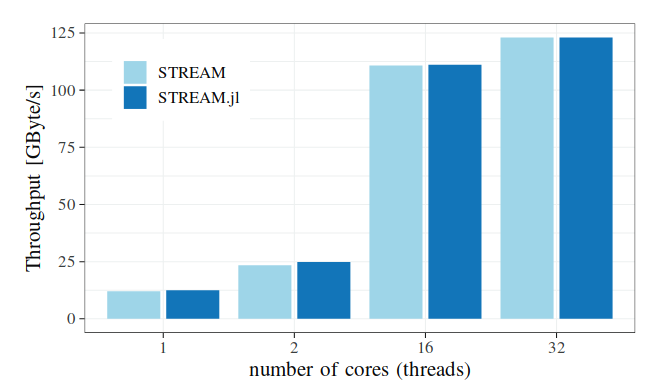
\includegraphics[width=10cm]{images/stream-1.png}
  \caption{Pengujian Pertama Menggunakan STREAM}
  \label{gambar stream-1}
  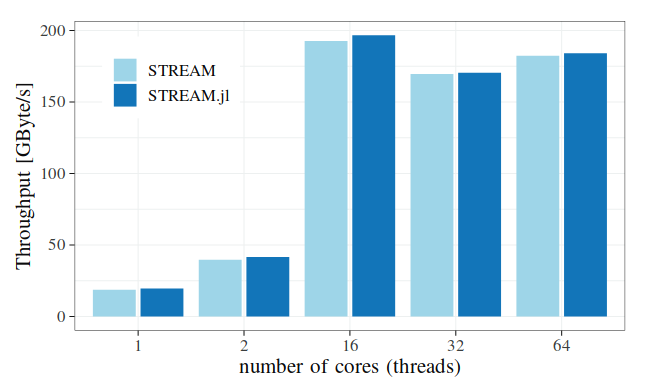
\includegraphics[width=10cm]{images/stream-2.png}
  \caption{Pengujian Kedua Menggunakan STREAM}
  \label{gambar stream-2}
\end{figure}

Penggunaan Julia pada sistem HPC (\emph{High Performance Computation}) perlu
diuji lebih lanjut. \cite{hunoldBenchmarkingJuliaCommunication2020} telah
melakukan penelitian penggunaan Julia pada sistem HPC.
\cite{hunoldBenchmarkingJuliaCommunication2020} menggunakan 2 metode pengukuran
HPC, yakni dengan STREAM yang mana dapat menjelaskan bagaimana performa sistem
untuk membaca/menulis pada \emph{Dynamic RAM} (DRAM), dan metode kedua adalah
dengan menggunakan ReproMPI yang mana menjelaskan bagaimana performa sistem
pada komunikasi data antar \emph{node}. Pada ReproMPI, terdapat 3 fungsi yang
digunakan, yakni \texttt{MPI\_Bcast}, \texttt{MPI\_Alltoall}, dan
\texttt{MPI\_Allreduce}. Hasil performa menggunakan Julia ini dibandingkan
dengan Bahasa C. Bahasa C ini memjadi acuan dikarenakan Bahasa C sudah terbukti
mampu untuk bekerja pada sistem HPC.

Pada Gambar \ref{gambar stream-1} dan \ref{gambar stream-2}, STREAM merupakan
simulasi yang ditulis dengan Bahasa C, sedangkan STREAM.jl merupakan simulasi
yang ditulis dengan Bahasa Julia. Dari kedua gambar tersebut, terlihat bahwa
Bahasa Julia mempunyai performa untuk membaca/menulis DRAM yang hampir seimbang
dengan Bahasa C.

\begin{figure}[H]
  \centering
  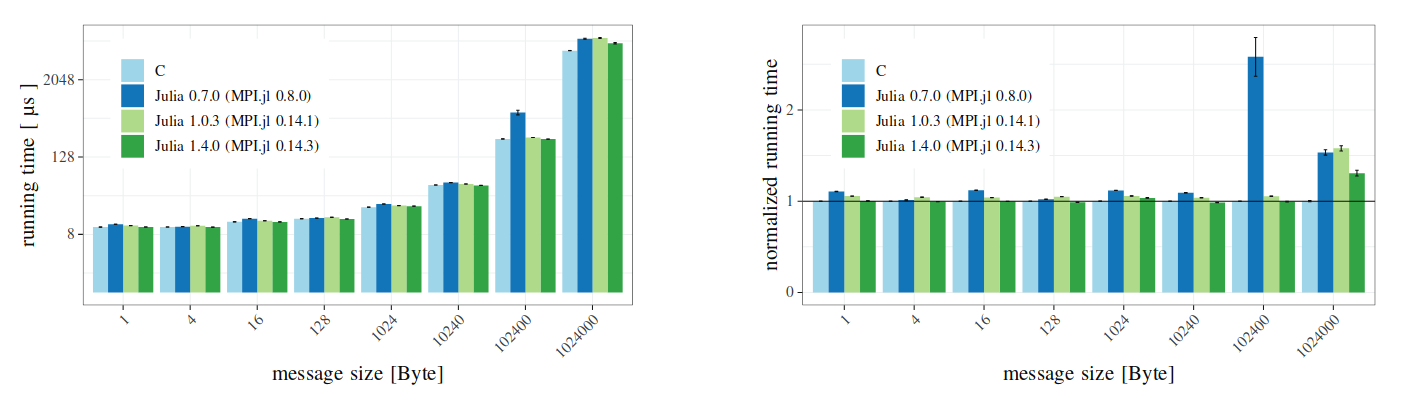
\includegraphics[width=14cm]{images/mpi-1.png}
  \caption{Pengujian Menggunakan MPI pada fungsi \texttt{MPI\_Bcast}}
  \label{gambar mpi-1 bcast}

  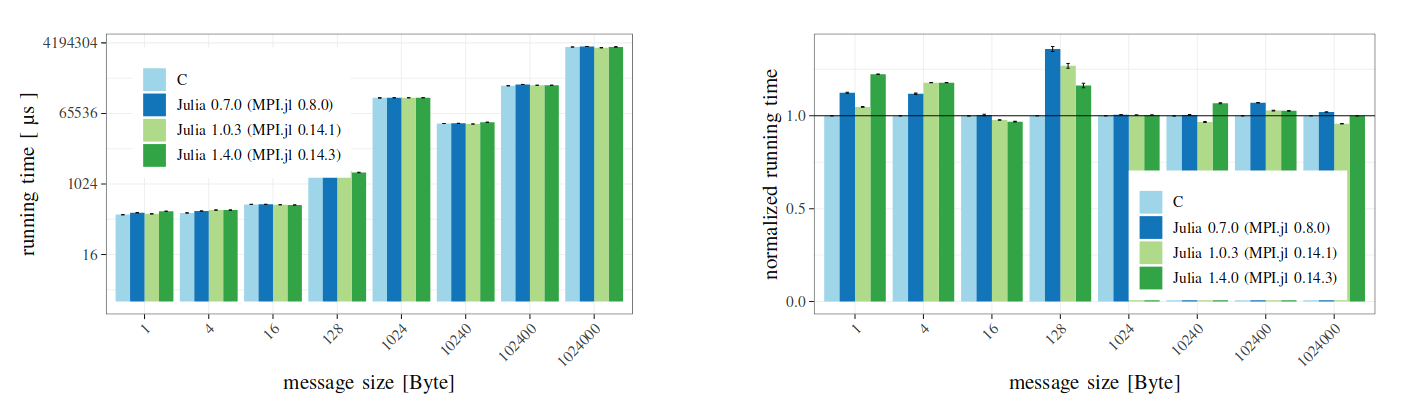
\includegraphics[width=14cm]{images/mpi-2.png}
  \caption{Pengujian Menggunakan MPI pada fungsi \texttt{MPI\_Alltoall}}
  \label{gambar mpi-2 alltoall}

  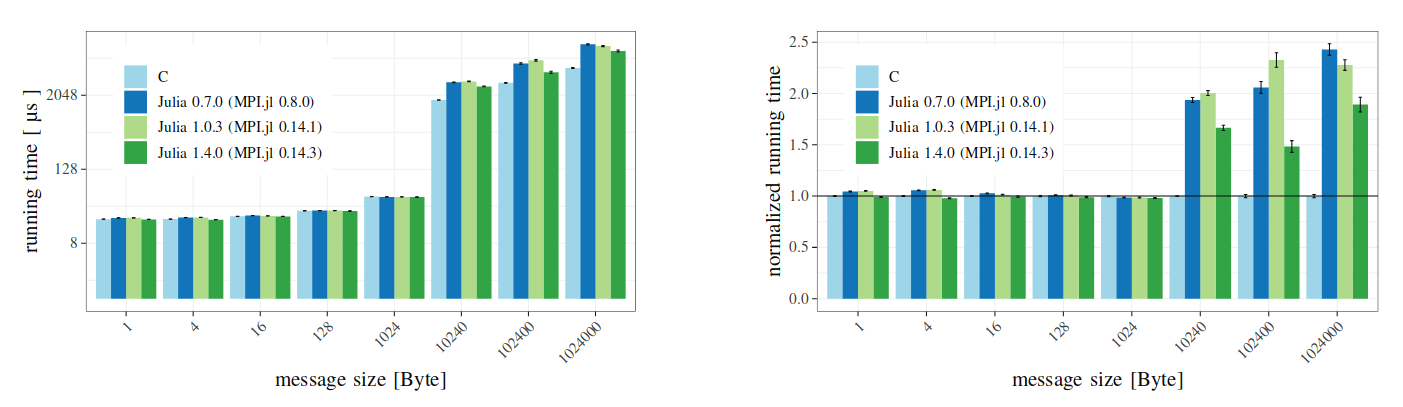
\includegraphics[width=14cm]{images/mpi-3.png}
  \caption{Pengujian Menggunakan MPI pada fungsi \texttt{MPI\_Allreduce}}
  \label{gambar mpi-3 allreduce}
\end{figure}

Pada Gambar \ref{gambar mpi-1 bcast}, \ref{gambar mpi-2 alltoall}, dan
\ref{gambar mpi-3 allreduce}, terlihat bahwa performa Bahasa Julia untuk
simulasi MPI umumnya memiliki nilai performa yang sama seperti Bahasa C.
Bahkan, sebenarnya untuk beberapa percobaan, performa Julia lebih baik daripada
C.

Dari kedua metode percobaan yang sudah dilakukan, dapat disimpulkan bahwa
performa Julia umumnya sama seperti C. Sehingga dapat dikatakan bahwa Julia
sudah bisa digunakan untuk sistem HPC.

\section{Pemrograman Julia dalam Komputasi Ilmiah}

Penggunaan Julia dalam komputasi ilmiah telah menjadi subjek penelitian yang
signifikan dalam beberapa tahun terakhir. Kemampuan Julia dalam menyeimbangkan
kinerja tinggi dan kemudahan pemrograman telah menjadikannya pilihan yang
menarik dalam berbagai bidang ilmiah. Berikut adalah tinjauan beberapa
literatur penting yang membahas aspek-aspek kunci dari penggunaan Julia dalam
komputasi ilmiah.

\cite{kulyabovComputerAlgebraJULIA2021} mengeksplorasi kemampuan Julia dalam aljabar
komputer. Hasil studi ini menunjukkan bagaimana Julia dapat digunakan untuk
komputasi simbolik dalam pemodelan matematis. \cite{kulyabovComputerAlgebraJULIA2021}
juga menyoroti bahwa Julia menawarkan sintaks yang sederhana dan kinerja yang memuaskan,
yang sangat bermanfaat dalam komputasi ilmiah. Kajian ini mendemonstrasikan kemampuan
Julia untuk mengintegrasikan komputasi numerik dan simbolik dalam satu kerangka kerja,
yang memungkinkan peneliti untuk melakukan analisis yang lebih kompleks dengan
efisiensi yang lebih tinggi.

\cite{tomasiNewSolutionsScientific2018} membahas fitur dan kekurangan Julia, serta
aplikasinya dalam astronomi dan astrofisika. Studi ini menekankan kecepatan
eksekusi yang tinggi dan ekspresifitas yang ditawarkan oleh Julia, yang mirip dengan
bahasa yang dikompilasi secara statis seperti C++ atau Fortran, sembari tetap
menyediakan shell interaktif dan dukungan penuh untuk Jupyter. Artikel ini membuktikan
bahwa Julia tidak hanya efisien dalam hal kinerja tetapi juga dalam hal produktivitas,
yang sangat penting dalam penelitian ilmiah.

\cite{zappanardelliJuliaSubtypingRational2018} memberikan definisi formal dari
relasi subtype dalam Julia dan memotivasi desainnya. Kajian ini penting karena menyoroti
bagaimana anotasi tipe pada deklarasi metode dalam Julia digunakan untuk memilih
metode yang paling tepat untuk sekumpulan argumen tertentu. Penelitian ini valid
secara empiris dengan implementasi definisi mereka yang dibandingkan dengan
implementasi Julia yang ada pada program dunia nyata. Temuan mereka menunjukkan keakuratan
dan efisiensi pendekatan subtyping Julia, yang sangat penting dalam pemrograman
multi-dispatch yang digunakan dalam komputasi ilmiah.

\cite{xiaoJuliaLanguageComputational2022b} melakukan survei komprehensif tentang
penggunaan bahasa Julia dalam mekanika komputasi. Penelitian ini menyoroti penggunaan
metode numerik dalam Julia dan menggambarkan bagaimana Julia memungkinkan peningkatan
abstraksi dan produktivitas. \cite{xiaoJuliaLanguageComputational2022b} membahas
kemampuan Julia dalam pengembangan paket perangkat lunak untuk mekanika
komputasi dan menantang penggunaan bahasa pemrograman yang lebih umum seperti
MATLAB atau Python dalam bidang ini. Studi ini menunjukkan bahwa Julia tidak hanya
efektif dalam hal kinerja tetapi juga dalam memberikan pendekatan yang lebih intuitif
untuk pemodelan dan simulasi dalam mekanika komputasi.

Kesimpulannya, Julia mempunyai kemampuan yang baik dalam komputasi ilmiah.
Julia menawarkan keseimbangan antara produktivitas dan kinerja. Dengan
kemampuan komputasi simbolik dan numeriknya, Julia tidak hanya meningkatkan
efisiensi dalam pemodelan dan analisis, tetapi juga mendukung inovasi dan
kemajuan dalam berbagai disiplin ilmiah.

% \section{Integrasi GPU dalam Fisika Komputasi}

% [Isinya berdasarkan metode]

% ==================================================

% \section{Komputasi Paralel dalam Fisika}

% \section{Perkembangan Terkini dalam GPU dan Julia}

% Penjelasan mengapa GPU lebih baik daripada CPU
% \section{Kinerja GPGPU}

% % Evolusi Pemrograman GPU:
% Komputasi GPU praktis dimulai dengan pengenalan CUDA (Compute Unified Device Architecture)
% oleh NVIDIA dan Stream oleh AMD, yang merupakan API (Application Programming
% Interface) yang dirancang untuk digunakan bersama dengan perangkat keras yang NVIDIA
% dan AMD sediakan. CUDA adalah sebuah platform dan model pemrograman yang
% memungkinkan para pengembang untuk menggunakan kekuatan komputasi GPU untuk
% proses yang lebih efisien dan canggih \citep{oanceaGPGPUComputing2014}.

% \begin{figure}[h]
%   \centering
%   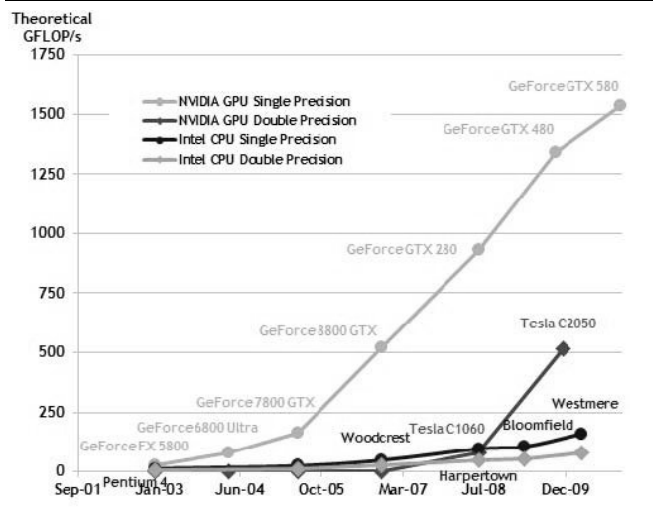
\includegraphics[width=10cm]{images/gpu-vs-cpu-flop-rates.png}
%   \caption{Tingkat FLOP teoritis dari GPU dan CPU}
%   \label{gambar flop rates gpu dan cpu}
% \end{figure}

% \cite{oanceaGPGPUComputing2014} menjelaskan bahwa \emph{flop rate} dari GPU dan CPU
% adalah seperti Gambar \ref{gambar flop rates gpu dan cpu}. Flop rate adalah
% ukuran kinerja yang menggambarkan seberapa cepat GPU dapat melakukan perhitungan
% matematika floating-point. Semakin tinggi flop rate, semakin cepat GPU dalam
% menyelesaikan operasi perhitungan yang kompleks. Terlihat pada Gambar \ref{gambar
% flop rates gpu dan cpu} bahwa perhitungan dengan menggunakan GPU mempunyai nilai
% teoritis flop rates yang jauh diatas CPU. Sehingga dapat disimpulkan bahwa GPU
% mempunyai kecepatan perhitungan kompleks yang jauh lebih tinggi daripada GPU.

% Sammy

% Pemelajaran mendalam (\emph{deep learning}) sebagai sebuah pemahaman telah lahir
% sejak tahun 1940an. Namun pemelajaran mendalam sebagai istilah yang tren memang
% baru muncul belakangan. Setidaknya ada tiga gelombang pengembangan pemelajaran mendalam
% yang ditandai dengan nomenklaturnya \citep{goodfellow_bengio_courville_2016}. Gelombang
% pertama (1940-1960an), istilah pemelajaran mendalam dikenal dengan \emph{cybernetics}
% yang merupakan pengembangan dari teori pola pemelajaran biologis \citep{mcculloch_pitts_1943, morris_1999}
% dan implementasi pertama pada model \emph{perceptron} \citep{rosenblatt_1958}.

% Pada gelombang kedua (1980-1995), dikenal dengan istilah \emph{connectionism}
% yang menggunakan pendekatan \emph{connectionist} dengan gebrakan baru yaitu perambatan
% mundur (\emph{back-propagation}) untuk melatih jaringan saraf (\emph{neural
% network}) dengan satu atau dua lapisan tersembunyi \citep{rumelhart_hinton_williams_1986}.
% Dan akhirnya gelombang ketiga atau masa kontemporer dimulai pada sekitar tahun 2006
% hingga sekarang yang dikenal dengan \emph{deep learning} \citep{hinton_osindero_teh_2006, NIPS2006_5da713a6}.

% Ilmu saraf memberikan wawasan yang banyak mengenai cara bekerja sebuah jaringan saraf
% biologis untuk dikembangkan ke dalam algoritma jaringan saraf buatan untuk belajar
% memecahkan beragam tugas yang berbeda \citep{goodfellow_bengio_courville_2016}. Salah
% satunya adalah penjelasan dari ilmuwan saraf bagaimana musang dapat belajar melihat
% dengan daerah pemrosesan pendengaran di otaknya jika otaknya diatur ulang untuk mengirimkan
% sinyal visual ke area tersebut \citep{von_melchner_pallas_sur_2000}. Hal ini kemudian
% menunjukkan bahwa mayoritas otak mamalia menggunakan algoritma tunggal untuk memecahkan
% kebanyakan tugas yang berbeda. Dari cara kerja tersebut, terinspirasilah ide utama
% untuk memiliki banyak unit komputasional yang menjadi pintar melalui interaksi dengan
% unit lain \citep{goodfellow_bengio_courville_2016}.

% Neocognitron \citep{fukushima_1980} memperkenalkan model arsitektur yang sangat bagus
% untuk memroses gambar yang terinspirasi dari sistem visual mamalia dan yang kemudian
% menjadi cikal bakal ide untuk pengembangan jaringan saraf konvolusi modern (\emph{modern
% convolutional neural network} \citep{726791, lecun_kavukcuoglu_farabet_2010}.

% Penyelesaian persamaan diferensial parsial menggunakan metode jaringan saraf
% buatan dimulai sejak tahun 1990an yang dimulai oleh \cite{lee_kang_1990} dengan
% artikelnya yang berjudul '\emph{Neural algorithm for solving differential
% equation}' yang terbit di \emph{Journal of Computational Physics}. Kemudian pada
% dekade yang sama muncul beberapa artikel yang membahas tentang topik ini, yaitu
% oleh Dissanayake dan Phan-Tien pada tahun 1994 dan Lagaris, dkk. pada tahun
% 1998.

% Dalam \citep{lagaris1998}, solusi persamaan diferensial dalam koordinat kartesian
% yang coba diselesaikan merupakan penjumlahan dari dua bagian. Bagian yang
% pertama merupakan permasalahan syarat batas atau syarat awal dan mengandung
% parameter yang tidak dapat diubah-ubah. Dan bagian yang kedua adalah bagian yang
% tidak memiliki hubungan dengan bagian syarat awal/syarat batas dan mengandung perambatan
% maju dari jaringan saraf buatan. Pengaplikasian metode ini dapat digunakan pada
% persamaan diferensial biasa tunggal, persamaan diferensial biasa berpasangan,
% dan persamaan diferensial parsial. Metode ini dikomparasikan dengan solusi dari metode
% numerik Galerkin \emph{finite element}.

% Usaha-usaha awal penggunaan jaringan saraf buatan pada penyelesaian persamaan
% diferensial parsial ini sangat memanfaatkan algoritma perambatan mundur karena
% memberikan metode yang sangat akurat untuk menghitung ralat. Namun usaha-usaha ini
% memiliki kendala yang kurang lebih sama, yaitu hanya mampu menangani fungsi ruas
% kanan dan syarat batas tertentu saja.

% Dengan perkembangan kekuatan komputasi pada tahun 2000an, dimungkinkan untuk membuat
% model yang lebih rumit, dan parameter yang lebih banyak, serta jumlah lapisan (\emph{layer})
% yang lebih banyak. \cite{Smaoui2004} menggunakan jumlah daya komputasional yang lebih
% besar untuk menginvestigasi model yang lebih mendalam. menggunakan \emph{multilayer
% perceptron} untuk memprediksi dinamika dari dua persamaan diferensial parsial nonlinear
% menggunakan dekomposisi Kahunen-Loeve dan jaringan saraf buatan.
% \cite{baymani2010} mengembangkan jaringan saraf buatan untuk penyelesaian
% permasalahan Stokes. Permasalahan Stokes campuran ditransformasi ke dalam tiga permasalahan
% Poisson koordinat kartesian yang kemudian diselesaikan untuk mendapatkan hasil dari
% permasalahan Stokes tersebut. Hasil yang didapat dari metode jaringan saraf
% buatan ini kemudian dikomparasikan dengan metode numerik dari penelitian lainnya
% dan hasil eksaknya. Dari penelitian tersebut didapatkan bahwa pendekatan jaringan
% saraf tiruan yang baru memberikan hasil yang memiliki akurasi yang lebih tinggi dan
% jumlah parameter yang digunakan lebih sedikit dari model konvensional.

% \cite{DBLP:journals/corr/abs-1711-10561} memperkenalkan jaringan saraf terinformasi
% fisika (\emph{physics informed neural networks} (PINN)), yaitu jaringan saraf yang
% dilatih untuk menyelesaikan tugas-tugas pembelajaran yang diawasi dengan tetap memperhatikan
% hukum fisika tertentu yang dijelaskan oleh persamaan diferensial parsial nonlinier
% umum. Pengembangan tersebut berada pada koridor untuk memecahkan dua masalah
% utama yaitu solusi berbasis data dan penemuan berbasis data dari persamaan
% diferensial parsial.

% Seiring dengan perkembangan model \emph{deep learning}, suatu terobosan dalam
% penyelesaian persamaan diferensial parsial menggunakan jaringan saraf buatan
% kemudian ditemukan. Para peneliti kemudian mengembangkan model jaringan saraf buatan
% konvolusi (\emph{convolutional neural network}/ CNN) dengan hipotesis bahwa dengan
% menggunakan CNN, parameter yang digunakan akan lebih sedikit sehingga akan
% banyak melakukan penghematan sumber daya komputer serta akan memberikan hasil
% yang lebih akurat. Selain itu, menurut \cite{Li_Li_Gao}, CNN memiliki kemampuan yang
% lebih baik untuk mengenali masukan gambar.

% \cite{shan_2020_study} mengembangkan model penyelesaian persamaan Poisson menggunakan
% CNN untuk memprediksi potensial listrik dengan variasi pada eksitasi dan distribusi
% permitivitas pada bidang kartesian 2 dimensi dan 3 dimensi. Penelitian ini
% menggunakan desain \emph{cost function} yang dikustomisasi dan data yang didapat
% dari metode numerik beda-hingga. Model yang dikembangkan dapat melakukan peforma
% yang cukup efektif dibandingkan dengan metode numerik yang digunakan untuk
% membentuk data latih, dengan rata-rata ralat prediksi kurang dari 3\%.

% Perkembangan yang cukup signifikan dilakukan oleh \cite{Ozbay2021} dengan
% mengembangkan arsitektur CNN untuk menyelesaikan persamaan Poisson 2 dimensi
% pada koordinat kartesian dengan variasi resolusi yang diberikan oleh ruas kanan
% persamaan, sembarang syarat batas, dan variasi parameter grid. Permasalahan syarat
% batas diselesaikan dengan metode baru, mendekomposisikan persaman Poisson yang
% asli ke dalam satu persamaan Poisson homogen dan empat submasalah Laplace
% nonhomogen. Model yang dikembangkan terbukti dapat mengungguli model dengan jaringan
% saraf tiruan konvensional dan dapat memprediksi dengan rata-rata presentase ralat
% di bawah 10\%.

% \cite{cheng2021using} menyelesaikan persamaan Poisson 2 dimensi dengan syarat
% batas Dirichlet nol menggunakan lapisan konvolusi secara penuh dengan arsitektur
% U-Net \citep{DBLP:journals/corr/RonnebergerFB15} yang didefinisikan dengan variasi
% pada jumlah percabangan, kedalaman, dan medan reseptif. Pada penelitian tersebut
% didapati bahwa medan reseptif memiliki peran yang penting dalam menangkap
% struktur topologis dari masukan pada tiap lapisan. Untuk menghitung syarat batas
% dan interior, digunakan dua syarat batas, yaitu \emph{dichlet loss} dan \emph{inside
% loss} serta syarat batas alternatif yaitu \emph{laplacian loss}. Untuk pelatihan
% digunakan dataset dengan distribusi muatan acak dan dataset dengan dengan distribusi
% mengikuti aturan deret Fourier.

% Sebagai domain fisis, dalam penelitian ini akan digunakan model pendorong Hall (\emph{Hall
% thruster}) sebagai perwakilan masalah fisis perhitungan potensial listrik di koordinat
% silinder. \cite{braga_miranda_2019} dari Laboratorium Fisika Plasma Universitas
% Brasil (LFP-UnB) sejak 2004 sedang mengembangkan pendorong Hall yang disebut
% PHall yang memiliki perbedaan dalam dimensi kanal, parameter operasi, dan
% mekanisme pembentukan medan magnet yang dibutuhkan dengan SPT-100. SPT-100
% dijadikan sebagai patokan dan pembanding dalam pembangunannya. Model 2 dimensi,
% spesifikasi serta, gambaran simulasi tentang SPT-100 dijelaskan dalam karya mereka.

% Penelitian ini akan memecahkan masalah persamaan diferensial parsial berupa persamaan
% Poisson yang diterapkan pada domain fisis pedorong Hall SPT-100 pada koordinat silinder
% dua dimensi menggunakan metode jaringan saraf konvolusi dengan \emph{ground
% truth} yang dihitung menggunakan metode numerik Gauss-Seidel.